\documentclass[10pt,oneside,twocolumn,a4paper]{article}
\usepackage[utf8]{inputenc}
\usepackage[T1]{fontenc}
\usepackage{amsmath}
\usepackage{tikz}
\usetikzlibrary{automata, positioning, arrows}
\tikzset{
    ->, % makes the edges directed
    >=stealth,
    node distance=4em, % specifies the minimum distance between two nodes. Change if necessary.
    every state/.style={thick, fill=gray!10, minimum size=4em}, % sets the properties for each ’state’ node
    initial text=$ $, % sets the text that appears on the start arrow
    fontscale/.style = {font=\scriptsize}
}
\usepackage{color}
\usepackage{xcolor}

\begin{document}

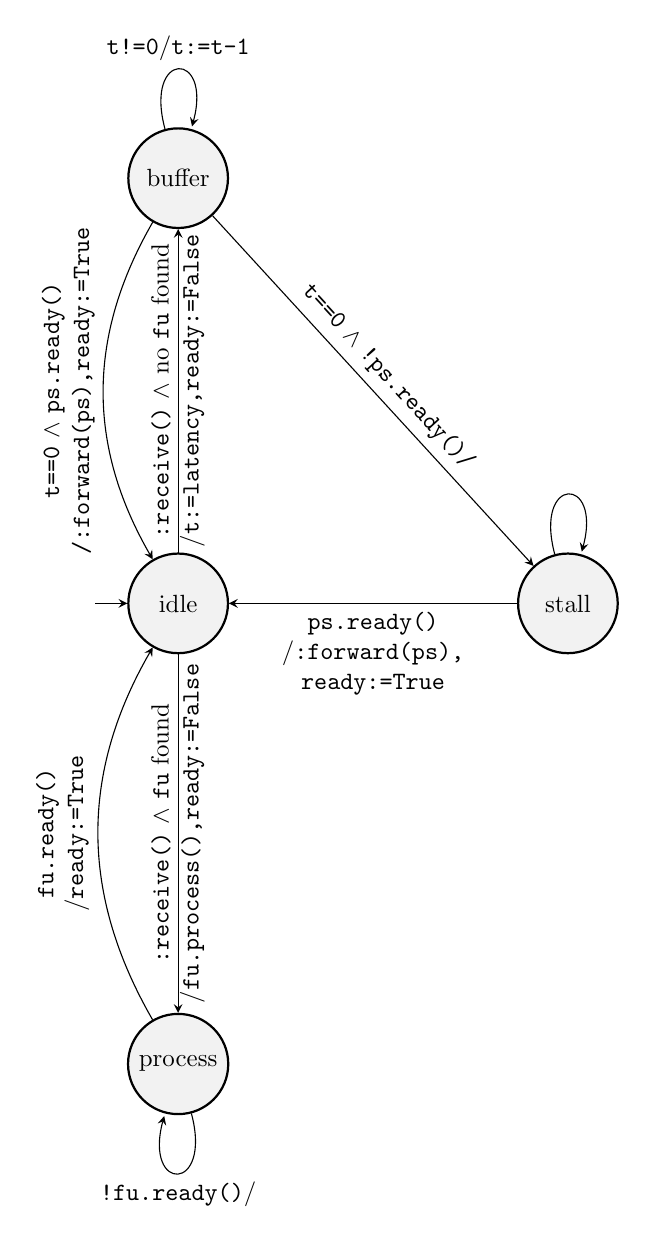
\begin{tikzpicture}[scale=0.9, every node/.style={scale=0.9}]
    \node[state, initial] at (0,6.5) (idle) {idle};
    \node[state] at (0,12.5) (buffer) {buffer};
    \node[state] at (0,0) (process) {process};
    \node[state] at (5.5,6.5) (stall) {stall};
    \draw   (idle) edge node[sloped, anchor=center, align=center] {\texttt{:receive()} $\wedge$ no \texttt{fu} found\\/\texttt{t:=latency,ready:=False}} (buffer)
            (buffer) edge[bend right] node[sloped, align=center, above, rotate=180] {\texttt{t==0} $\wedge$ \texttt{ps.ready()}\\\texttt{/:forward(ps),ready:=True}} (idle)
            (idle) edge node[sloped, anchor=center, align=center, rotate=180] {\texttt{:receive()} $\wedge$ \texttt{fu} found\\/\texttt{fu.process(),}\texttt{ready:=False}} (process)
            (process) edge[bend left] node[sloped, anchor=center, align=center,above] {\texttt{fu.ready()}\\/\texttt{ready:=True}} (idle)
            (buffer) edge node[sloped, anchor=center, above, align=center] {\texttt{t==0} $\wedge$ \texttt{!ps.ready()/}} (stall)
            (stall) edge node[align=center, below] {\texttt{ps.ready()}\\/\texttt{:forward(ps),}\\\texttt{ready:=True}} (idle)
            (stall) edge[loop above] node {} (stall)
            (buffer) edge[loop above] node {\texttt{t!=0}/\texttt{t:=t-1}} (buffer)
            (process) edge[loop below] node {\texttt{!fu.ready()}/} (process)
    ;
\end{tikzpicture}

\end{document}